\documentclass{beamer}[10]

\usepackage{graphicx}
\usepackage{xcolor}
\usepackage{tabto}
%\usepackage{beamerthemesplit}
\usepackage{tikz}
\usepackage{cancel}
\usepackage{verbatim}
\usepackage{fancybox}
\usepackage{enumerate}
\usepackage{amsmath,amssymb,amsthm,textcomp,mathtools}
\usepackage[super]{nth}
\usepackage[amssymb]{SIunits}
\usepackage{booktabs}
\usepackage{cancel}
\usepackage{bm}
\usepackage[utf8]{inputenc}
\usepackage{tabularx}
\usepackage{ragged2e}
\newcolumntype{Y}{ >{\RaggedRight\arraybackslash}X}
\usetikzlibrary{arrows,shapes}
\newcommand\T{\rule{0pt}{2.6ex}}
\newcommand\B{\rule[-1.2ex]{0pt}{0pt}}
\definecolor{UUcrimson}{RGB}{204,0,0}
\mode<presentation>
{ \usetheme{default}
  \usecolortheme[named=UUcrimson]{structure}
  \useinnertheme{circles}
  \setbeamercovered{transparent}
  \setbeamertemplate{blocks}[rounded]
  \usefonttheme[onlymath]{serif}
  \setbeamertemplate{navigation symbols}{}
  \setbeamertemplate{footline}[page number]
  \setbeamertemplate{navigation symbols}{}
  \setbeamercolor{section in toc}{fg=black,bg=white}
  \setbeamercolor{alerted text}{fg=UUcrimson!80!gray}
  \setbeamercolor*{palette primary}{fg=white,bg=UUcrimson}
  \setbeamercolor*{palette secondary}{fg=UUcrimson!70!black,bg=gray!15!white}
  \setbeamercolor*{palette tertiary}{bg=UUcrimson!80!black,fg=gray!10!white}
  \setbeamercolor*{palette quaternary}{fg=UUcrimson,bg=gray!5!white}
  \setbeamercolor*{palette sidebar primary}{fg=UUcrimson!10!black}
  \setbeamercolor*{palette sidebar secondary}{fg=white}
  \setbeamercolor*{palette sidebar tertiary}{fg=UUcrimson!50!black}
  \setbeamercolor*{palette sidebar quaternary}{fg=gray!10!white}
  \setbeamercolor{titlelike}{parent=palette primary,fg=white}
  \setbeamercolor{frametitle}{bg=UUcrimson}
  \setbeamercolor{frametitle right}{bg=UUcrimson}
  \setbeamercolor*{separation line}{}
  \setbeamercolor*{fine separation line}{}
}

\usetikzlibrary{backgrounds}
\makeatletter
\tikzstyle{every picture}+=[remember picture]
\tikzset{%
  fancy quotes/.style={
    text width=\fq@width pt,
    align=justify,
    inner sep=1em,
    anchor=north west,
    minimum width=\linewidth,
    font=\itshape
  },
  fancy quotes width/.initial={.8\linewidth},
  fancy quotes marks/.style={
    scale=8,
    text=white,
    inner sep=0pt,
  },
  fancy quotes opening/.style={
    fancy quotes marks,
  },
  fancy quotes closing/.style={
    fancy quotes marks,
  },
  fancy quotes background/.style={
    show background rectangle,
    inner frame xsep=0pt,
    background rectangle/.style={
      fill=gray!25,
      rounded corners,
    },
  }
}
\newenvironment{fancyquotes}[1][]{%
\noindent
\tikzpicture[fancy quotes background]
\node[fancy quotes opening,anchor=north west] (fq@ul) at (0,0) {``};
\tikz@scan@one@point\pgfutil@firstofone(fq@ul.east)
\pgfmathsetmacro{\fq@width}{\linewidth - 2*\pgf@x}
\node[fancy quotes,#1] (fq@txt) at (fq@ul.north west) \bgroup}
{\egroup;
\node[overlay,fancy quotes closing,anchor=east] at (fq@txt.south east) {''};
\endtikzpicture}
\makeatother

\usepackage{scalerel}[2014/03/10]
\usepackage{stackengine}
\usepackage{empheq}
\newcommand*\widefbox[1]{\fbox{\hspace{0.5em}#1\hspace{0.5em}}}

\newcommand\reallywidetilde[1]{\ThisStyle{%
  \setbox0=\hbox{$\SavedStyle#1$}%
  \stackengine{-.1\LMpt}{$\SavedStyle#1$}{%
    \stretchto{\scaleto{\SavedStyle\mkern.2mu\sim}{.5467\wd0}}{.4\ht0}%
%    .2mu is the kern imbalance when clipping white space
%    .5467++++ is \ht/[kerned \wd] aspect ratio for \sim glyph
  }{O}{c}{F}{T}{S}%
}}
\usepackage{media9}

\logo{
\includegraphics[width=0.75cm]{logo.jpg}}
\author[Gibbs]{Dr. Jeremy A. Gibbs}
\institute{Department of Mechanical Engineering\\University of Utah}
\date{Fall 2016}
\title{LES of Turbulent Flows: Lecture 2}
\begin{document}

%----------------------------------------------------------------------------------------
%	TITLE & TOC SLIDES
%----------------------------------------------------------------------------------------

\begin{frame} 
  \titlepage
\end{frame}

%------------------------------------------------

\begin{frame}
\frametitle{Overview}
\tableofcontents
\end{frame}

%------------------------------------------------
\section{Basic Properties of Turbulence} %
%------------------------------------------------
\begin{frame}{Basic Properties of Turbulence}
\begin{itemize}
\item \textbf{Turbulence is random} \newline The properties of the fluid ($\rho$, $P$, $u$) at any given point ($x$,$t$) cannot be predicted. But statistical properties – time and space averages, correlation functions, and probability density functions – show regular behavior. The fluid motion is stochastic.
\item \textbf{Turbulence decays without energy input} \newline Turbulence must be driven or else it decays, returning the fluid to a laminar state.
\end{itemize}
\end{frame}

%------------------------------------------------

\begin{frame}{Basic Properties of Turbulence}
\begin{itemize}
\item \textbf{Turbulence displays scale-free behavior} \newline On all length scales larger than the viscous dissipation scale but smaller than the scale on which the turbulence is being driven, the appearance of a fully developed turbulent flow is the same.
\item \textbf{Turbulence displays intermittency} \newline ``Outlier'' fluctuations occur more often than chance would predict.
\end{itemize}
\end{frame}
%------------------------------------------------

\begin{frame}{Basic Properties of Turbulent Flows}
\setlength{\fboxsep}{0pt}
\setlength{\fboxrule}{1pt}
\begin{columns}[T]
    \begin{column}{.65\textwidth}
      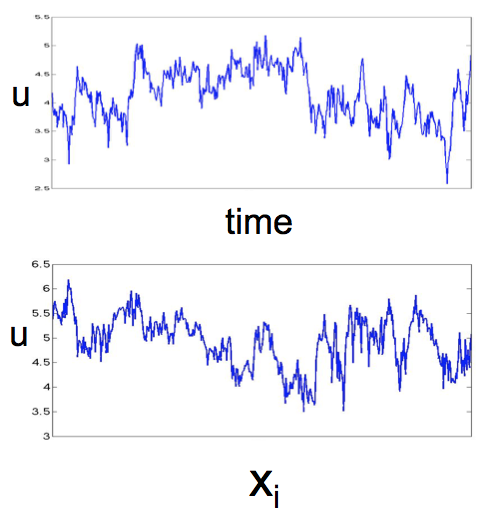
\includegraphics[width=\textwidth]{timetrace2.png}
    \end{column}
    \begin{column}{.35\textwidth}
    \begin{minipage}[c][.7\textheight][c]{\linewidth}
    \begin{itemize}
      \item Unsteady\newline\newline\newline\newline\newline\newline
      \item Three-dimensional	
      \end{itemize}
      \end{minipage}
    \end{column}
  \end{columns}

\end{frame}

%------------------------------------------------

\begin{frame}{Basic Properties of Turbulent Flows}
\begin{itemize}
\item Large vorticity\newline\newline
\item Vorticity describes the tendency of something to rotate.
\begin{align*}
\omega &= \nabla \times \vec{u}\\
&= \epsilon_{ijk}\frac{\partial}{\partial x_i}u_j \hat{e}_k\\
&= \left(\frac{\partial u_3}{\partial x_2} - \frac{\partial u_2}{\partial x_3}\right)\hat{e}_1 + \left(\frac{\partial u_1}{\partial x_3} - \frac{\partial u_3}{\partial x_1}\right)\hat{e}_2 + \left(\frac{\partial u_2}{\partial x_1} - \frac{\partial u_1}{\partial x2}\right)\hat{e}_3
\end{align*}
~\\
Vortex stretching can and does create small scale circulations that increases the turbulence intensity $I$, where:
$$I = \frac{\sigma_u}{\langle u \rangle}$$
\end{itemize}
\end{frame}

%------------------------------------------------

\begin{frame}{Basic Properties of Turbulent Flows}
\begin{itemize}
\item Mixing effect\newline\newline
Turbulence mixes quantities (\textit{e.g.}, pollutants, chemicals, velocity components, etc)., which acts reduce gradients. This lowers the concentration of harmful scalars, but increases drag.
\item A continuous spectrum (range) of scales.
\begin{figure}
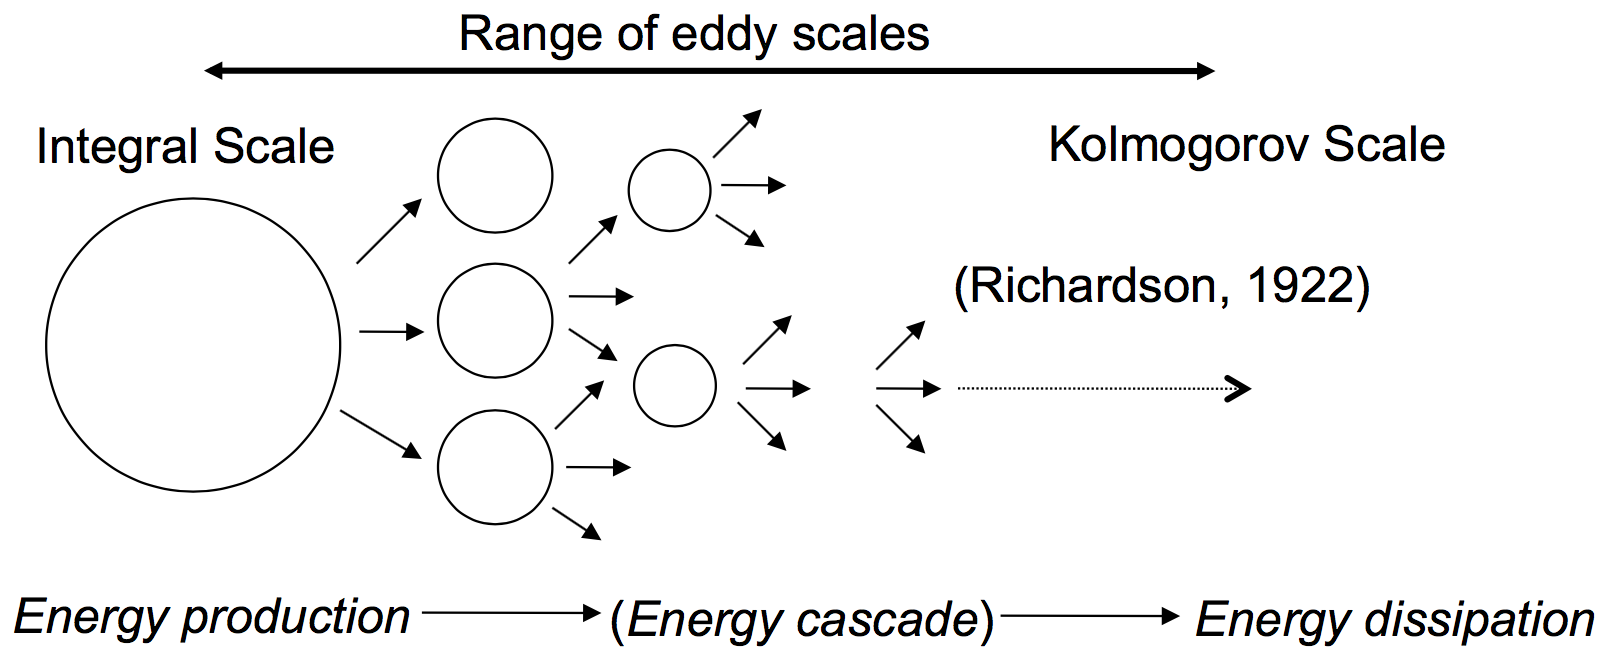
\includegraphics[width=0.9\textwidth]{scales}	
\end{figure}
\end{itemize}
\end{frame}

%------------------------------------------------
\section{Random Nature of Turbulence} %
%------------------------------------------------

\begin{frame}{Random Nature of Turbulence}
  \begin{figure}[H]
  \centering
  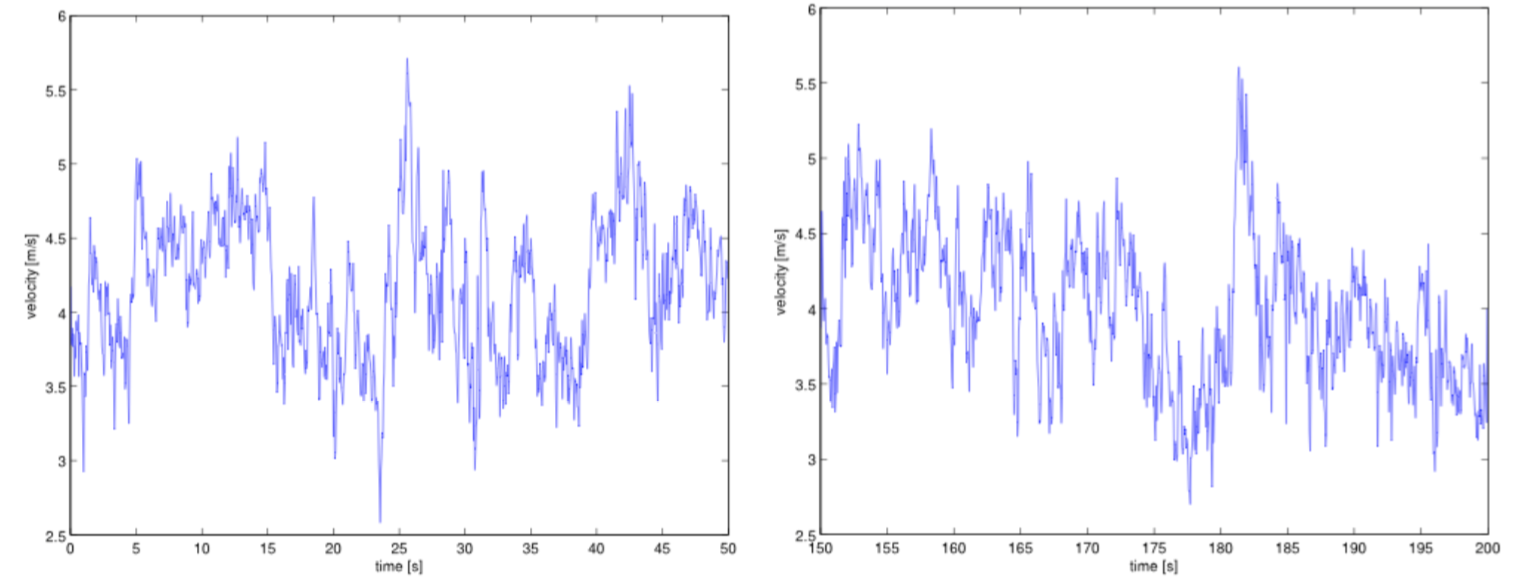
\includegraphics[width=1\textwidth]{timetrace1.png}
  \caption{\scriptsize Sonic anemometer data at 20Hz taken in the ABL.}
  \end{figure}
  
  This velocity field exemplifies the random nature of turbulent flows.
\end{frame}

%------------------------------------------------

\begin{frame}{Random Nature of Turbulence}
  \begin{figure}[H]
  \centering
  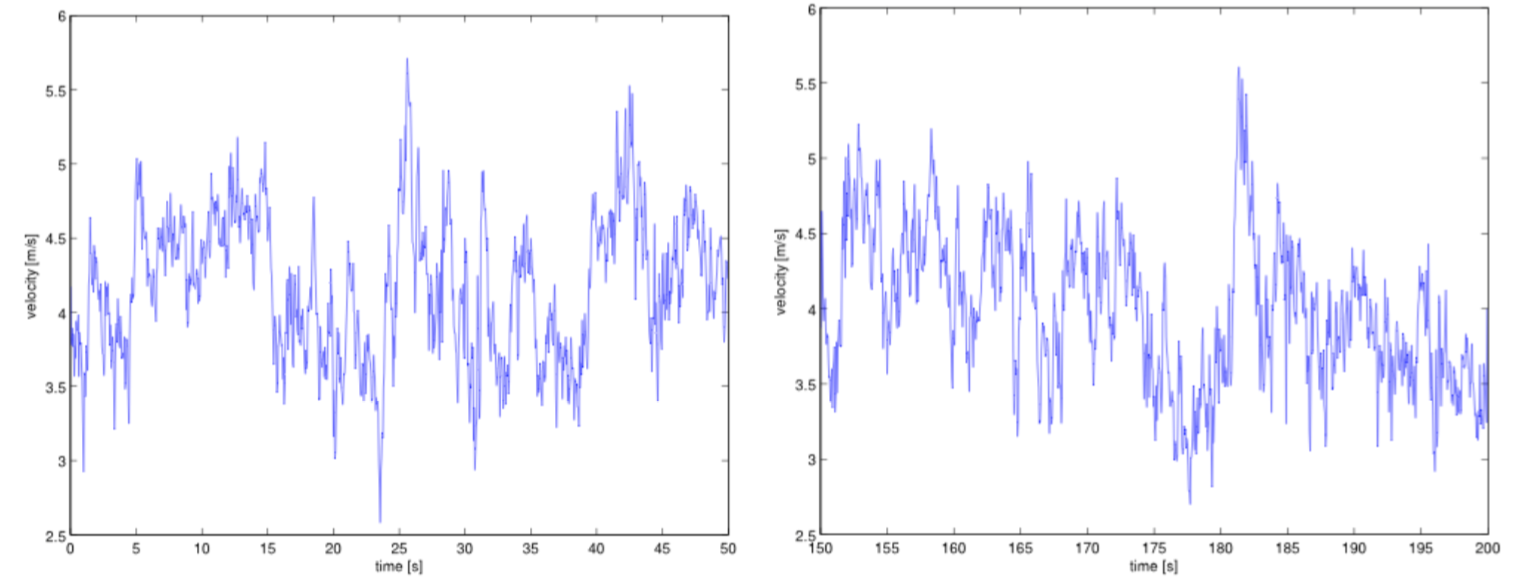
\includegraphics[width=1\textwidth]{timetrace1.png}
  \end{figure}
  \begin{itemize}
  \item The signal is highly disorganized and has structure on a wide range of scales (that is also disorganized).\newline\newline Notice the small (fast) changes verse the longer timescale changes that appear in no certain order.
  \end{itemize}
\end{frame}

%------------------------------------------------

\begin{frame}{Random Nature of Turbulence}
  \begin{figure}[H]
  \centering
  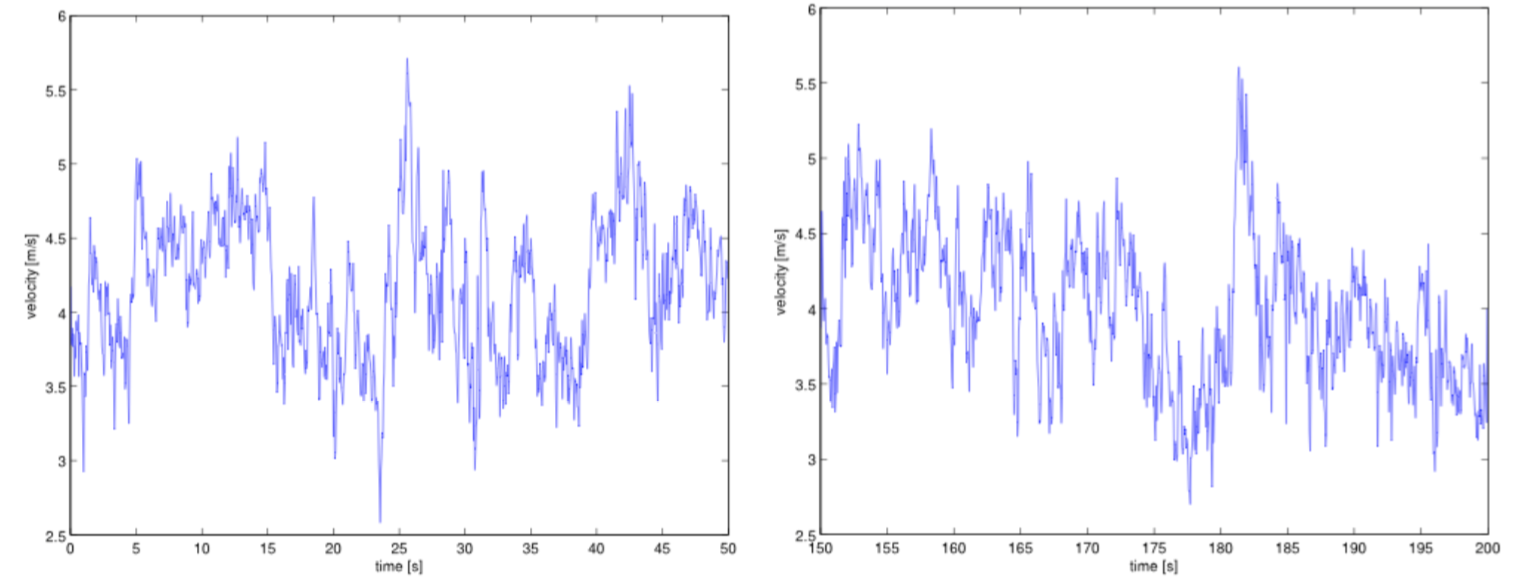
\includegraphics[width=1\textwidth]{timetrace1.png}
  \end{figure}
  \begin{itemize}
  \item The signal appears unpredictable.\newline\newline Compare the left plot with that on the right ($100$ s later). Basic aspects are the same but the details are completely different. From looking at the left signal, it is impossible to predict the right signal.
  \end{itemize}
\end{frame}

%------------------------------------------------

\begin{frame}{Random Nature of Turbulence}
  \begin{figure}[H]
  \centering
  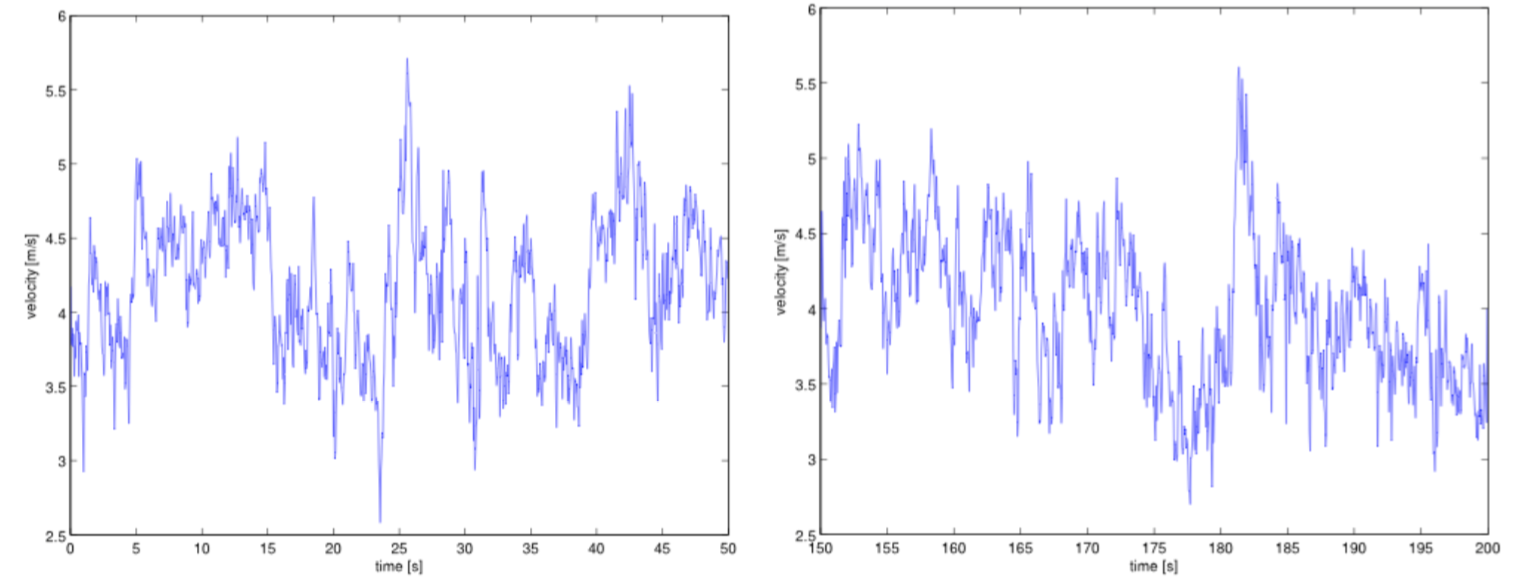
\includegraphics[width=1\textwidth]{timetrace1.png}
  \end{figure}
  \begin{itemize}
  \item Some of the properties of the signal appear to be reproducible.\newline\newline The reproducible property isn't as obvious from the signal. Instead we need to look at the histogram.
  \end{itemize}
\end{frame}


%------------------------------------------------

\begin{frame}{Random Nature of Turbulence}
  \begin{figure}[H]
  \centering
  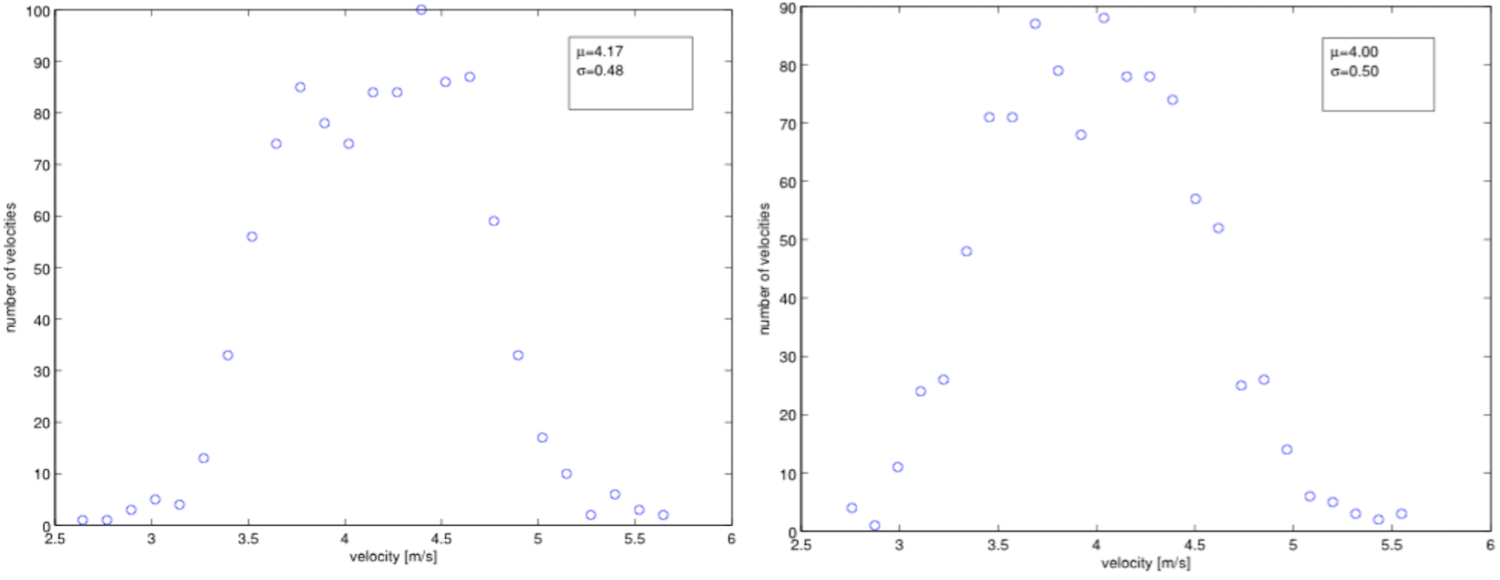
\includegraphics[width=1\textwidth]{histogram.png}
  \end{figure}
  Notice that the histograms are similar with similar means and standard deviations.
\end{frame}

%------------------------------------------------

\begin{frame}{Random Nature of Turbulence}
\setlength{\fboxsep}{0pt}
\setlength{\fboxrule}{1pt}
\begin{columns}[T]
    \begin{column}{.35\textwidth}
      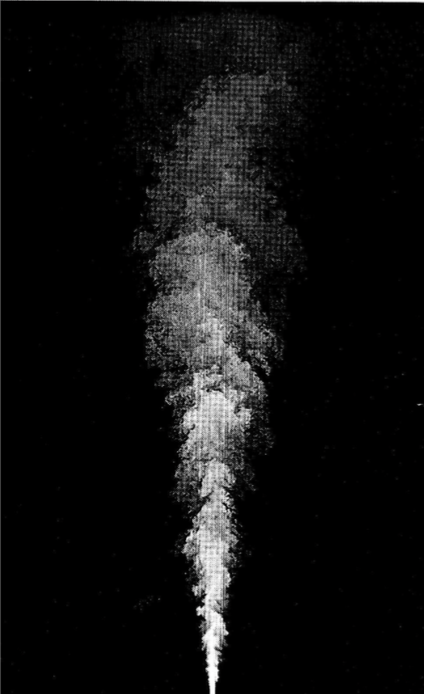
\includegraphics[width=\textwidth]{jet.png}
    \end{column}
    \begin{column}{.65\textwidth}
    \begin{minipage}[c][.7\textheight][c]{\linewidth}
    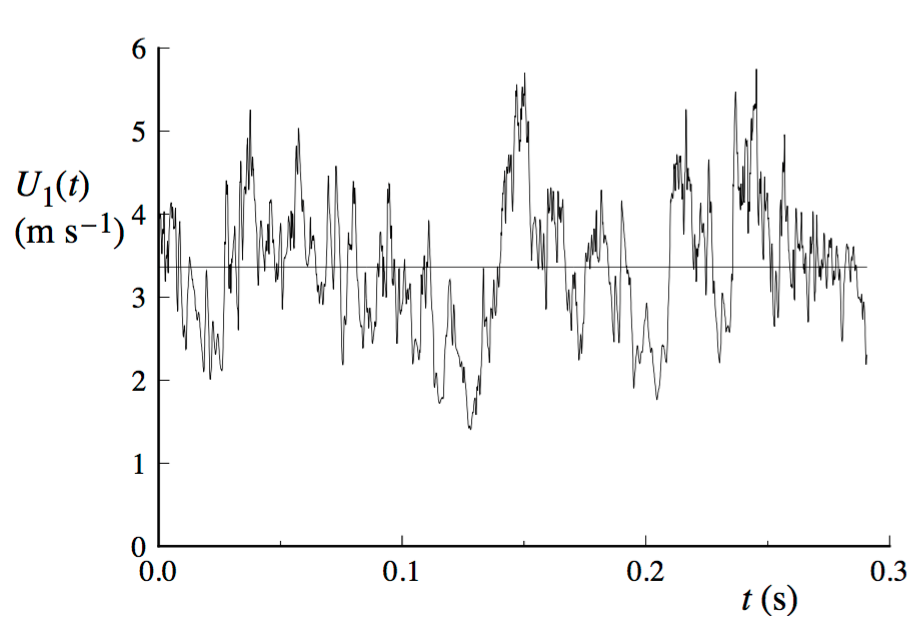
\includegraphics[width=\textwidth]{timetrace3.png}
    \end{minipage}
    \end{column}
  \end{columns}
  The left panel shows concentration in a turbulent jet, while the right shows the time history along the centerline (see Pope).
\end{frame}

%------------------------------------------------

\begin{frame}{Random Nature of Turbulence}
  \begin{figure}[H]
  \centering
  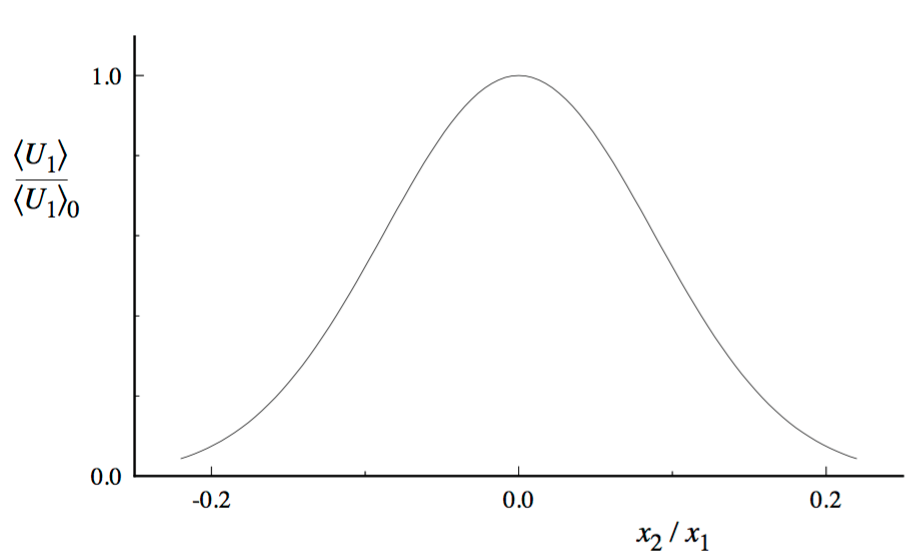
\includegraphics[width=1\textwidth]{crossu.png}
  \end{figure}
  Normalized mean axial velocity in a turbulent jet (see Pope).
\end{frame}

%------------------------------------------------

\begin{frame}{Random Nature of Turbulence}
  \begin{itemize}
  	\item The random behavior observed in the time series can appear to contradict what we know about fluids from classical mechanics.
  	\item The Navier-Stokes equations are deterministic (\textit{i.e.}, they give us an exact mathematical description of the evolution of a Newtonian fluid).
  	\item Yet, as we have seen, turbulent flows are random.
  	\item How do we resolve this inconsistency?
  \end{itemize}
\end{frame}

%------------------------------------------------

\begin{frame}{Random Nature of Turbulence}
  Question: Why the randomness?
  \begin{itemize}
  	\item There are unavoidable perturbations (\textit{e.g.}, initial conditions, boundary conditions, material properties, forcing, etc.) in turbulent flows.
  	\item Turbulent flows and the Navier-Stokes equations are acutely sensitive to these perturbations.
  	\item These perturbations do not fully explain the random nature of turbulence, since such small changes are present in laminar flows.
  	\item However, the sensitivity of the flow field to these perturbations at large Re is much higher.
  \end{itemize}
\end{frame}

%------------------------------------------------

\begin{frame}{Random Nature of Turbulence}
  \begin{itemize}
  	\item This sensitivity to initial conditions has been explored extensively from the viewpoint of dynamical system. This is often referred to as chaos theory.
  	\item The first work in this area was carried out by Lorenz (1963) in the areas of atmospheric turbulence and predictability. Perhaps you have heard the colloquial phrase, \textit{the butterfly effect}.
  	\item Lorenz studied a system with three state variables $x$, $y$, and $z$ (see his paper or Pope for details). He ran one experiment with $x(0) = 1$ and another with $x=1.000001$, while $y$ and $z$ were held constant.
  \end{itemize}
\end{frame}

%------------------------------------------------

\begin{frame}{Random Nature of Turbulence}
  \begin{figure}[H]
  \centering
  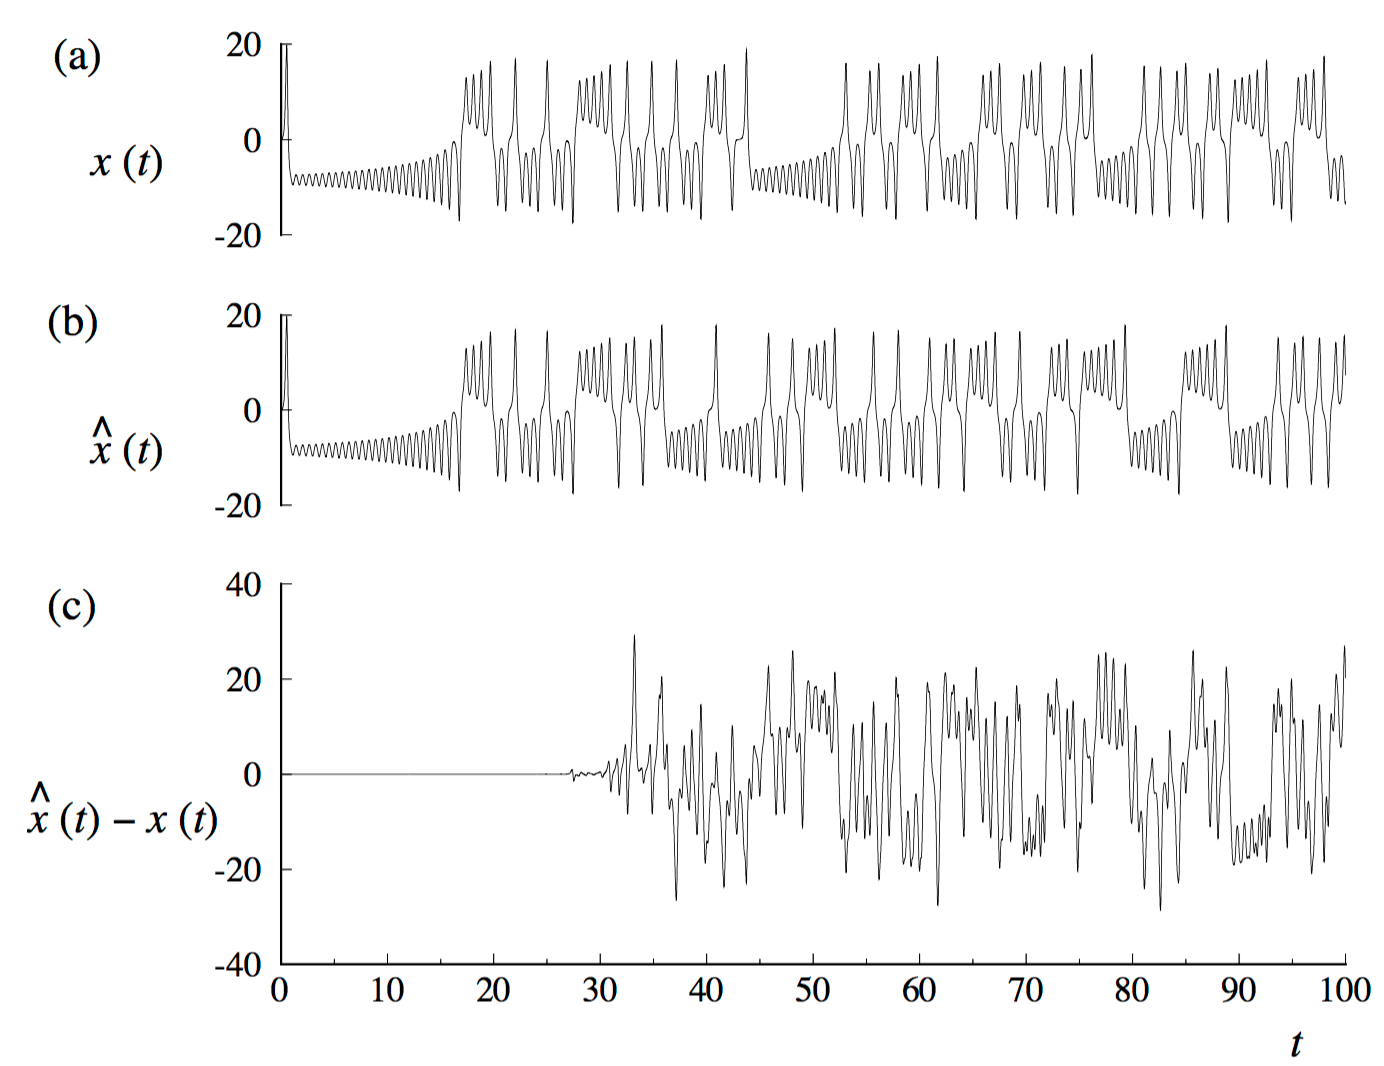
\includegraphics[width=0.85\textwidth]{lorenz.png}
  \caption{Time history of the Lorenz equations.}
  \end{figure}
\end{frame}

%------------------------------------------------

\begin{frame}{Random Nature of Turbulence}
  \begin{itemize}
  	\item The work by Lorenz demonstrates the extreme sensitivity to initial conditions.
  	\item The result of this sensitivity is that beyond some point, the state of the system cannot be predicted (\textit{i.e.}, the limits of predictability).
  	\item In the Lorenz example, even when the initial state is known to within $10^{-6}$, predictability is limited to $t = 35$.
  \end{itemize}
\end{frame}

%------------------------------------------------

\begin{frame}{Random Nature of Turbulence}
  \begin{itemize}
  	\item In the Lorenz example, this behavior depends on the coefficients of the system. If a particular coefficient is less than some critical value, the solutions are stable. If, on the other hand, it exceeds that value, then the system becomes chaotic.
  	\item This is similar to the Navier-Stokes equations, where solutions are steady for a sufficiently small Re, but turbulent if Re becomes large enough.
  \end{itemize}
\end{frame}

%------------------------------------------------

\begin{frame}{Random Nature of Turbulence}
  \begin{itemize}
  	\item We have seen that turbulent flows are random, but their histograms are apparently reproducible.
  	\item As a consequence, turbulence is usually studied from a statistical viewpoint.
  \end{itemize}
\end{frame}

%------------------------------------------------
\section{Statistical Tools for Turbulent Flow} %
%------------------------------------------------
\begin{frame}{Basic Properties of Turbulence}
\begin{itemize}
  	\item Consider the velocity field $U$.
  	\item Since $U$ is a random variable, its value is unpredictable for a turbulent flow.
  	\item Thus, any theory used to predict a particular value for $U$ will likely fail.
  	\item Instead, theories should aim at determining the probability of events (\textit{e.g.}, $U < 10\ \metre\ \reciprocal\second$).
  	\item We need statistical tools to characterize random variables.
  \end{itemize}
\end{frame}

%------------------------------------------------

\begin{frame}{Sample Space}
\begin{itemize}
  	\item In reality, a velocity field $U(\vec{x},t)$ is more complicated than a single random variable.
  	\item In order to consider more general events than our example of $U < 10\ \metre\ \reciprocal\second$, we need to think in terms of \textit{sample space}.
  	\item Consider an independent velocity variable $V$, which is the sample-space variable for $U$.
  \end{itemize}
\end{frame}

%------------------------------------------------

\begin{frame}{Sample Space}
  \begin{figure}[H]
  \centering
  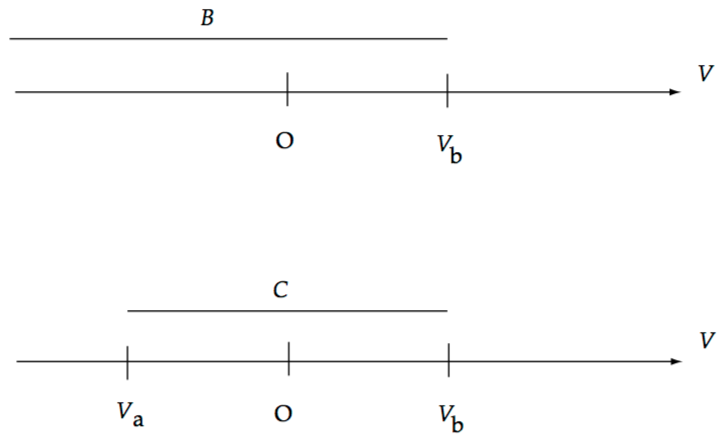
\includegraphics[width=0.65\textwidth]{samplespace.png}
  \end{figure}
  \begin{align*}
  B &\equiv \{U < V_b \}\\C &\equiv \{V_a \leq U < V_b \}
  \end{align*}
  $B$ and $C$ are events (or values) that correspond to different regions of the sample space (\textit{i.e.}, velocity field).
  
\end{frame}

%------------------------------------------------

\begin{frame}{Probability}
\begin{itemize}
  	\item Using the previous example, the probability of event $B$ is given as:
  	$$p=P(B)=P\{U<V_b\}$$
  	\item This is the likelihood of $B$ occurring ($U<V_b$).
  	\item $p$ is a real number, $0 \leq p \leq 1$.
  	\item $p = 0$ is an impossible event.
  	\item $p = 1$ is a certain event.
  \end{itemize}
\end{frame}

%------------------------------------------------

\begin{frame}{Cumulative Distribution Function}
\begin{itemize}
  	\item The probability of any event is determined by the cumulative distribution function (CDF)
  	$$F(V) \equiv P\{U<V\}$$
  	\item For event $B$:
  	$$P(B) = \{U < V_b \} = F(V_b)$$
  	\item For event $C$:
  	\begin{align*}
  	P(C) &= \{V_a \leq U < V_b \} = P\{U < V_b \} - P\{U < V_a \}\\ &= F(V_b) - F(V_a)
  	\end{align*}
  \end{itemize}
\end{frame}

%------------------------------------------------

\begin{frame}{Cumulative Distribution Function}
Three basic properties of CDF:
\begin{itemize}
  	\item $F(-\infty) = 0$, since $\{U < -\infty\}$ is impossible.
  	\item $F(\infty) = 1$, since $\{U > \infty\}$ is impossible.
  	\item $F(V_b) \geq F(V_a)$, for $V_b > V_a$, since $p > 0$. Thus, $F$ is a non-decreasing function.  
  \end{itemize}
\end{frame}

%------------------------------------------------

\begin{frame}{Probability Density Function}
The probability density function (PDF) is the derivative of the CDF
$$f(V)\equiv \frac{d F(v)}{dV}$$
Based on the properties of the CDF, it follows that:
\begin{itemize}
  	\item $f(V) \geq 0$
  	\item $\int^{\infty}_{-\infty} f(V) dV = 1$
  	\item $f(-\infty) = f(\infty) = 0$
  \end{itemize}
\end{frame}

%------------------------------------------------

\begin{frame}{Probability Density Function}

The probability that a random variable is contained within a specific interval is the integral of the PDF over that interval 
\begin{align*}
P(C) = P\{V_a \leq U < V_b \} &= F(V_b) - F(V_a)\\
&= \int^{V_b}_{V_a} f(V) dV
\end{align*}

Or, for a very small interval $dV_s$:
\begin{align*}
P(C_s) = P\{V_a \leq U < V_a + dV_s \} &= F(V_a + dV_s) - F(V_a)\\
&= f(V_a)dV_s
\end{align*}

\end{frame}

%------------------------------------------------

\begin{frame}{Probability Density Function}
More details about the PDF $f(V)$:
\begin{itemize}
	\item $f(V)$ is the probability per unit distance in the sample space -- hence, the term \textit{density}.
	\item $f(V)$ has dimensions of $U^{-1}$, while the CDF is dimensionless.
	\item The PDF fully characterizes the statistics of a signal (random variable).
	\item If two or more signals have the same PDF, then they are considered to be statistically identical.
	\end{itemize}
\end{frame}

%------------------------------------------------

\begin{frame}{CDF (top) vs. PDF (bottom)}
  \begin{figure}[H]
  \centering
  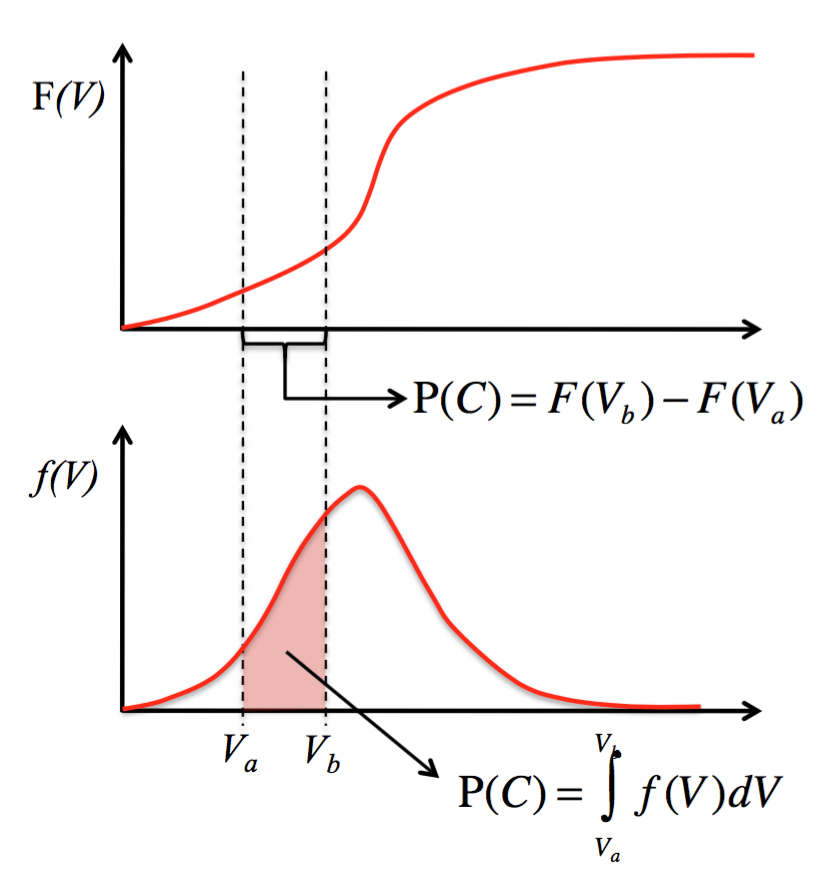
\includegraphics[width=0.7\textwidth]{cdfpdf.png}
  \end{figure}
\end{frame}

%------------------------------------------------

\begin{frame}{Means and Moments}
We can also define a signal by its individual statistics, which collectively describe the PDF.
~\\~\\
The mean (or expected) value of a random variable $U$ is given by:
$$\langle U \rangle \equiv \int^{\infty}_{-\infty} Vf(V)dV$$
or in discrete form:
$$\langle U \rangle \equiv \frac{1}{N} \sum^N_{i=1} V_i$$
The mean represents the probability-weighted sum of all possible values of $U$.
\end{frame}

%------------------------------------------------

\begin{frame}{Means}
Consider some function of $U$, $Q(U)$.

$$\langle Q(U) \rangle \equiv \int^{\infty}_{-\infty} Q(V)f(V)dV$$

The mean $\langle Q(U) \rangle$ only exists if the above integral converges absolutely. From this equation, we can show that for $Q(U)$, $R(U)$, and constants $a$ and $b$:

$$\langle aQ(U) + bR(U) \rangle = a\langle Q(U) \rangle +  b\langle R(U) \rangle$$

Thus, $\langle \; \rangle$ behave as a linear operator.

\end{frame}

%------------------------------------------------

\begin{frame}{Means}

Although $U$, $Q(U)$, and $R(U)$ are random variables, $\langle U \rangle$, $\langle Q(U) \rangle$, and $\langle R(U) \rangle$ are not.\newline\newline Thus, the mean of the mean is just the mean (\textit{i.e.}, $\langle \langle U \rangle \rangle = \langle U \rangle$).

\end{frame}

%------------------------------------------------

\begin{frame}{Variance}

Let's define a \textit{fluctuation} (or perturbation) from the mean:
$$u^\prime \equiv U - \langle U \rangle$$
The \textit{variance} is just the mean-square fluctuation:
\begin{align*}
\sigma_u^2 = \text{var}(U) &= \langle {u^\prime}^2 \rangle\\
&= \int^{\infty}_{-\infty} (V - \langle U \rangle)^2 f(V) dV 
\end{align*}
Or, in discrete form:
$$\sigma_u^2 = \frac{1}{N-1^*} \sum^N_{i=1} (V_i - \langle U \rangle)^2$$

Variance essentially measures how far a set of (random) numbers are spread out from their mean.
\newline\newline
\scriptsize{$^*$note the ($N-1$). This is the \href{https://en.wikipedia.org/wiki/Bessel\%27s_correction}{\color{UUcrimson}\underline{Bessel correction}} -- used to correct for bias.}

\end{frame}

%------------------------------------------------

\begin{frame}{Standard Deviation}

The \textit{standard deviation}, or root-mean square (rms) deviation, is just the square-root of the variance:
$$\sigma_u \equiv \text{sdev}(U) = \sqrt{\sigma_u^2} = \langle {u^\prime}^2 \rangle^{0.5}$$

The standard deviation basically measures the amount of variation of a set of numbers.
\end{frame}

%------------------------------------------------

\begin{frame}{Other moments}

The $n^{th}$ central moment is defined as:
$$\mu_n \equiv \langle {u^\prime}^n \rangle = \int^{\infty}_{-\infty} (V - \langle U \rangle)^n f(V)dV$$
\end{frame}

%------------------------------------------------

\begin{frame}{Standardized Moments}

It is often advantageous to express variables as standardized random variables. These standardized variables have zero mean and unit variance.\newline\newline
The standardized version of $U$ (centered and scaled) is given by:
$$\hat U \equiv \frac{U - \langle U \rangle}{\sigma_u}$$
Accordingly, the $n^{th}$ standardized moments are expressed as:
$$\hat \mu_n \equiv \frac{\langle {u^\prime}^n \rangle}{\sigma_u^n} = \frac{\mu_n}{\sigma_u^n}  = \int^{\infty}_{-\infty} \hat V^n \hat f(\hat V)d \hat V$$

\end{frame}

%------------------------------------------------

\begin{frame}{Other moments}

Different moments each describe an aspect of the shape of the PDF:
\begin{itemize}
	\item $\mu_1$      = mean (expected value)
	\item $\mu_2$      = variance (spread from the mean)
	\item $\hat \mu_3$ = skewness (asymmetry of PDF)
	\item $\hat \mu_4$ = kurtosis (sharpness of the PDF peak)
\end{itemize}

\end{frame}

%------------------------------------------------

\begin{frame}{Example PDFs}

Read Pope (Chapter 3.3) for descriptions of different PDFs. \newline\newline Examples include:
\begin{itemize}
	\item uniform
	\item exponential
	\item Gaussian
	\item log-normal
	\item gamma
	\item Delta-function
	\item Cauchy
\end{itemize}

\end{frame}

%------------------------------------------------

\begin{frame}{Joint Random Variables}

So far, our statistical description has been limited to single random variables. However, turbulence is governed by the Navier-Stokes equations, which are a set of 3 coupled PDEs.\newline\newline
We expect this will result in some correlation between different velocity components.

\end{frame}

%------------------------------------------------

\begin{frame}{Joint Random Variables}
  Example: turbulence data from the ABL: scatter plot of horizontal (u) and vertical (w) velocity fluctuations.
  \begin{figure}[H]
  \centering
  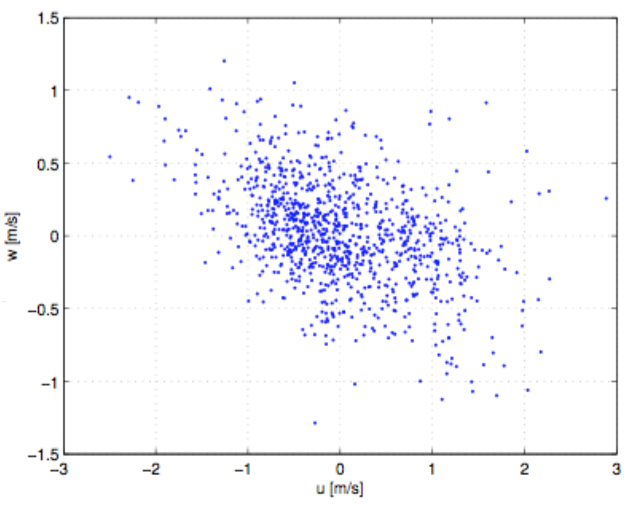
\includegraphics[width=0.7\textwidth]{jr1.png}
  \end{figure}
  The plot appears to have a pattern (\textit{i.e.}, negative slope).
\end{frame}

%------------------------------------------------

\begin{frame}{Joint Random Variables - Sample Space}
  We will now extend the previous results from a single velocity component to two or more.\newline\newline
  The sample-space variables corresponding to the random variables $U=\{U_1,U_2,U_3\}$ are given by $V=\{V_1,V_2,V_3\}$.
\end{frame}

%------------------------------------------------

\begin{frame}{Joint Random Variables - CDF}
  
  \setlength{\fboxsep}{0pt}
\setlength{\fboxrule}{1pt}
\begin{columns}[T]
    \begin{column}{.55\textwidth}
    \begin{minipage}[c][.6\textheight][c]{\linewidth}
    The joint CDF (jCDF) of the random variables ($U_1, U_2$) is given by:
  $$F_{12}(V_1,V_2) \equiv P\{U_1 < V_1, U_2 < V_2\}$$
  This is the probability of the point ($V_1,V_2$) lying inside the shaded region 
      \end{minipage}
    \end{column}
    \begin{column}{.55\textwidth}
      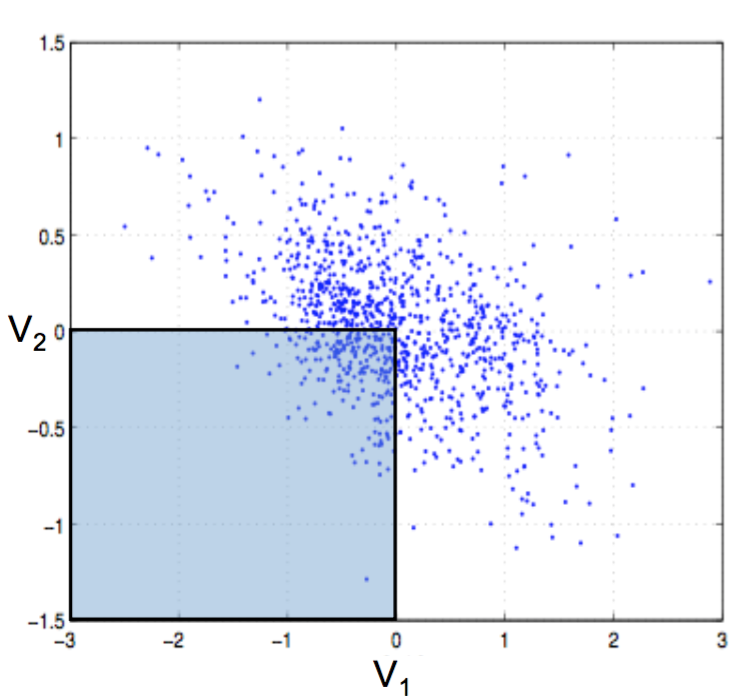
\includegraphics[width=\textwidth]{jr2.png}
    \end{column}
  \end{columns}
  
\end{frame}

%------------------------------------------------

\begin{frame}{Joint Random Variables - CDF}
  The jCDF has the following properties:
  
  \begin{itemize}
  	\item $F_{12}(V_1 + \delta V_1, V_2 + \delta V_2) \geq F_{12}(V_1, V_2)$ (non-decreasing) \newline for all $\delta V_1\geq0$, $\delta V_2\geq0$\newline
  	\item $F_{12}(-\infty,V_2) = P\{U_1<-\infty,U_2<V_2\} = 0$\newline since $\{U_1 < -\infty\}$ is impossible.\newline
  	\item $F_{12}(\infty,V_2) = P\{U_1<\infty,U_2<V_2\} = P\{U_2<V_2\}\newline F_{12}(\infty,V_2) = F_2(V_2)$, since $\{U_1 < \infty\}$ is certain.\newline
  \end{itemize}

  In the last example, $F_2(V_2)$ is called the \textit{marginal CDF}.
\end{frame}

%------------------------------------------------

\begin{frame}{Joint Random Variables - PDF}
  The joint PDF (jPDF) is defined as:
  $$f_{12}(V_1, V_2) \equiv \frac{\partial^2}{\partial V_1 \partial V_2}F_{12}(V_1,V_2)$$
  If we integrate over $V_1$ and $V_2$, we get the probability:
  $$P\{V_{1a} \leq U_1 < V_{1b}, V_{2a} \leq U_2 < V_{2b}\} = \int^{V_1b}_{V_1a} \int^{V_2b}_{V_2a} f_{12}(V_1,V_2)dV_2dV_1$$
  
\end{frame}

%------------------------------------------------

\begin{frame}{Joint Random Variables - PDF}
  Based on the jCDF, the jPDF has the following properties:
  \begin{itemize}
  	\item $f_{12} (V_1,V_2) \geq 0$\newline
  	\item $\int^{\infty}_{-\infty} f_{12}(V_1,V_2)dV_1 = f_2(V_2)$\newline
  	\item $\int^{\infty}_{-\infty} \int^{\infty}_{-\infty} f_{12}(V_1,V_2)dV_1dV_2 = 1$\newline
  \end{itemize}
  
  In the middle example, $f_2(V_2)$ is called the \textit{marginal PDF}. Practically speaking, we find the PDF of a time (or space) series by:
  \begin{itemize}
  	\item Create a histogram of the series(group values into bins)
  	\item Normalize the bin weights by the total \# of points
  \end{itemize}
\end{frame}

%------------------------------------------------

\begin{frame}{Joint Random Variables - Means}
  
  Similar to the single variable form, if we have $Q(U_1,U_2)$:
  $$\langle Q(U_1,U_2) \rangle \equiv \int^{\infty}_{-\infty} \int^{\infty}_{-\infty} Q(V_1,V_2)f_{12}dV_2dV_1$$
  We can use this equation to define a few important statistics.
  
\end{frame}

%------------------------------------------------

\begin{frame}{Joint Random Variables - Covariance}
  We can define \textit{covariance} as:
  \begin{align*}
  \text{cov}(U_1,U_2) &\equiv \newline \langle u_1^\prime u_2^\prime \rangle \\ &= \int^{\infty}_{-\infty} \int^{\infty}_{-\infty}(V_1 - \langle U_1 \rangle)(V_2 - \langle U_2 \rangle) f_{12}(V_1,V_2)dV_2dV_1
  \end{align*}
  Or for discrete data
  \begin{align*}
  \text{cov}(U_1,U_2) &\equiv \langle u_1^\prime u_2^\prime \rangle \\ &= \frac{1}{N-1} \sum^N_{j-1} (V_{1j} - \langle U_1 \rangle)(V_{2j} - \langle U_2 \rangle)
  \end{align*}
  Covariance is basically a measure of how much two random variables change together.
\end{frame}

%------------------------------------------------

\begin{frame}{Joint Random Variables - Correlation Coefficient}
  
  The \textit{correlation coefficient} is given by:
  $$\rho_{12} \equiv \frac{\langle u_1^\prime u_2^\prime \rangle}{\sqrt{\langle {u_1^\prime}^2\rangle \langle {u_2^\prime}^2 \rangle}}$$
  Correlation coefficient has the following properties:
  \begin{itemize}
  	\item $-1 \leq \rho_{12} \leq 1$
  	\item Positive values indicate correlation.
  	\item Negative values indicate anti-correlation.
  	\item $\rho_{12} = 1$ is perfect correlation.
  	\item $\rho_{12} = -1$ is perfect anti-correlation.
  \end{itemize}
\end{frame}

%------------------------------------------------

\begin{frame}{Two-point Statistical Measures}
  
  \textit{Autocovariance} measures how a variable changes with different lags, $s$.
  $$R(s) \equiv \langle u(t) u(t+s)\rangle$$
  or the \textit{autocorrelation function}
  $$\rho(s) \equiv \frac{ \langle u(t)u(t+s)\rangle}{u(t)^2}$$
  Or for the discrete form
  $$\rho(s_j) \equiv \frac{ \sum^{N-j-1}_{k=0}(u_ku_{k+j})}{\sum^{N-1}_{k=0}(u_k^2)}$$
  
\end{frame}

%------------------------------------------------

\begin{frame}{Two-point Statistical Measures}
  
  Notes on autocovariance and autocorrelation
  \begin{itemize}
  	\item These are very similar to the covariance and correlation coefficient
  	\item The difference is that we are now looking at the linear correlation of a signal with itself but at two different times (or spatial points), i.e. we lag the series.
  	\item We could also look at the cross correlations in the same manner (between two different variables with a lag).
  	\item $\rho(0) = 1$ and $|\rho(s)| \leq 1$
  \end{itemize}
  
\end{frame}
%------------------------------------------------

\begin{frame}{Two-point Statistical Measures}
  
\setlength{\fboxsep}{0pt}
\setlength{\fboxrule}{1pt}
\begin{columns}[T]
    \begin{column}{.45\textwidth}
    \begin{itemize}
    	\item In turbulent flows, we expect the correlation to diminish with increasing time (or
distance) between points
    	\item We can use this to define an integral time (or space) scale. It is defined as the time lag where the integral $\int \rho(s)ds$ converges. 
    	\item It can also be used to define the largest scales of motion (statistically).
    \end{itemize}
    \end{column}
    \begin{column}{.55\textwidth}
    \begin{minipage}[c][.6\textheight][c]{\linewidth}
      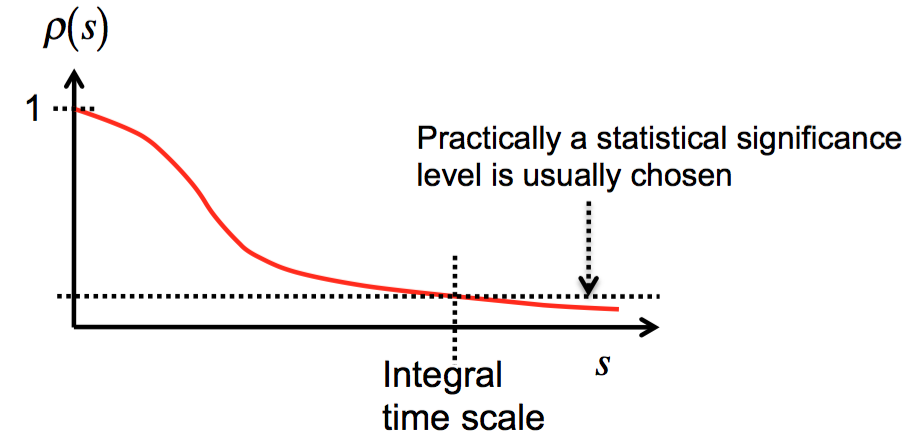
\includegraphics[width=\textwidth]{auto1.png}
      \end{minipage}
    \end{column}
  \end{columns}
  
\end{frame}

%------------------------------------------------

\begin{frame}{Two-point Statistical Measures}
  
  The \textit{structure function} is another important two-point statistic.
  $$D_n(r) \equiv \langle [U_1(x+r,t) - U_1(x,t)]^n\rangle$$
  \begin{itemize}
  	\item This gives us the average difference between two points separated by a distance $r$ raised to a power $n$.
  	\item In some sense it is a measure of the moments of the velocity increment PDF.
  	\item Note the difference between this and the autocorrelation which is statistical linear correlation (\textit{i.e.}, multiplication) of the two points.
  \end{itemize}
  
\end{frame}

%------------------------------------------------

\end{document}

